\documentclass[../thesis.tex]{subfiles}

\begin{document}

\chapter{Linking Predictive and Prescriptive Analytics for Healthcare Services}\label{chp:Linking}

\section{Introduction}
Predictive and prescriptive modelling are two powerful techniques in OR that have the ability to extract insights and guide decision makers. Predictive models are used to forecast future outcomes based on historical data and patterns, while prescriptive models provide recommendations on how to optimise those outcomes based on certain constraints and objectives. While both techniques are valuable in their own right, they become even more powerful when linked together. By integrating predictive and prescriptive models, organisations can only predict future outcomes, and also make informed decisions on how to optimise those outcomes in the most effective and efficient ways possible. This can lead to more accurate and impactful decision making, and ultimately improve business and healthcare performance. The concept of linking these two methods is still relatively novel, \cite{Lopes2020,Williams2022}, especially within the healthcare field and has great potential to drive significant value for organisations across a wide range of industries.

\begin{description}
\item[\textcolor{red}{Research Aim}] - This Chapter aims to link the CART results with deterministic and two-stage stochastic models together to ensure the results are consistent. It will seek to present the results in order to address the following research objective: `How can linking predictive and prescriptive analytics increase the reliability of the models?'.
\end{description}

The remainder of the Chapter is structured as follows: Section \ref{sec:linking} discuses linking the predictive and prescriptive paradigms together. Section \ref{sec:scenarioanalysis} determines the robustness of the models by applying a number of different scenarios. Section \ref{sec:generalization} discusses the flexibility within the models which allows users to apply them to other healthcare situations.

%\section{Linking Paradigms}

%One of the four research aims is to determine `how can linking predictive and prescriptive analytics increase the reliability of the models?'. 
%This Chapter aims to link the CART results with deterministic and two-stage stochastic models together to ensure the results are consistent.
\section{Linking Paradigms}\label{sec:linking}
To investigate linking these two paradigms, two methods have been explored and applied to both the classification tree and regression tree results. The first method used each end node to calculate the number of patients of each specialty using the average LOS from each end node. The second approach used each end node and the specific LOS for each specialty and hospital within the node. These were then summed together to form the D$_{s,r}$ parameter. These two methods were run on both the regression and the classification trees, using the Microsoft Excel implementation. The results have been compared on a year to year basis, as well as the three year range. Similar to previous experiments, the models have been run with a maximum run time of 100 seconds and a tolerance of 0.01\%. The VSS was calculated using the deterministic and two-stage stochastic models. The demands utilised within this section and the resulting heatmaps can be seen within Appendix \ref{app:linkeddemands}.
%Two methods will be explored, firstly by using each end node and determining the number of patients of each specialty and hospital using the average LOS from each end node. The second method will take each end node and the specific LOS for each specialty and hospital within the node. These will then be summed together to form the D$_{s,r}$ parameter. These two methods will be run on both the regression and the classification trees, using the Microsoft Excel implementation. The results will be compared on a year to year basis, as well as a three year range. Similar to previous experiments, the models will be run with a maximum run time of 100 seconds and a tolerance of 0.01\%. The deterministic and two-stage stochastic models will be used to calculated the VSS. The demands utilised within this section and the resulting heatmaps can be seen within Appendix \ref{app:linkeddemands}.

\subsection{Regression Tree and Average LOS}
The first method utilised the regression tree generated in Section \ref{sec:regressiontrees} (Figure \ref{fig:finalregtree}). This tree generated 30 patient groupings determined by the 30 leaf nodes. The average LOS determined by each node was used to calculate the demand for each node. Using Equation \eqref{eq:treedemand1}, the average demand was calculated as follows:

\begin{equation}\label{eq:treedemand1}
        D_{s,r} = \sum\limits_{h \in r} D_{s,h} = \frac{\text{Number of Patients}_{s,h}*\text{Node Average LOS}}{1096}
\end{equation}

The procedure for calculating the average bed demand for node two is shown in Table \ref{tab:Node2Regression}. For reference, on Figure \ref{sec:regressiontrees}, node two is the second left leaf node, and it indicates if a patient meets any of the eleven criteria listed below:
\begin{enumerate}
    \item Admission method $\neq$ Other - transferred from another hospital
    \item Admission method $\neq$ Elective - waiting list
    \item Admission method $\neq$ Elective - booked
    \item Specialty $\neq$ Accident \& Emergency
    \item Admission method $\neq$ Elective - planned
    \item Hospital $\neq$ Ysbyty Ystrad Fawr
    \item Age Group $\neq$ 65 - 69
    \item Age Group $\neq$ 70 - 74
    \item Specialty $\neq$ Trauma \& Orthopaedic
    \item Age Group $\neq$ 75 - 79
    \item Specialty = Care Of The Elderly
\end{enumerate}

For this end node, there were three hospitals included, all of which were the COTE specialty accounting for 8,776 patients. The final column of Table \ref{tab:Node2Regression} refers to the average daily bed demand across three years' worth of data. Each node's demands are consolidated for each specialty and hospital and then used for the overall demand, and are shown within Table \ref{apptab:LinkedDemands1}.
\begin{table}[h!]
    \centering\scalebox{0.8}{
    \begin{tabular}{ccccc}\toprule 
    \textbf{Hospital} & \textbf{Specialty} & \textbf{Count}& \textbf{Average LOS} & \textbf{Average Daily Demand}\\\midrule
    Nevill Hall Hospital &  Care Of The Elderly &     2696 &11.393 & 28.0251168 \\
    Royal Gwent Hospital &  Care Of The Elderly &     6076 & 11.393& 63.1604635 \\
    Ysbyty Aneurin Bevan &  Care Of The Elderly &        4 & 11.393&  0.0415803\\ \bottomrule
    \end{tabular}}
    \caption{Regression Tree Node Two - Average LOS}
    \label{tab:Node2Regression}
\end{table}


Table \ref{tab:Results1} presents the results from the demands generated using the average LOS. These demands can be found within Table \ref{tab:LinkedDemands1} in the Appendix. The same four scenarios, as listed in Table \ref{tab:scenarios1}, were applied to the demand figures. The VSS can be calculated to be 2.79\% with a saving of $\pounds$29,062.78. In comparison to the Table \ref{tab:eiveesveevdettwostageresults1}, there was a difference in deterministic solution of approximately 0.27\%, with the regression tree deploying fewer numbers of beds and nurses. The number of beds deployed in the first stage of the two-stage stochastic model does not change, but their locations do. % The differences in the objective function, bed and staff deployment could be due to the regression tree R$^{2}$ score of 34.28\% which is not accounting for longer LOS's. 

\begin{table}[h!]
    \centering
    \begin{tabular}{cccccl}\toprule
 & \multicolumn{2}{l}{\textbf{Total Beds}} & \multicolumn{2}{c}{\textbf{Total Staff}} & \multirow{2}{*}{\textbf{Objective Value ($\pounds$)}}\\ \cmidrule(lr){2-3} \cmidrule(lr){4-5}
 & xbed           & ubed          & xstaff         & ustaff         \\ \midrule
    Deterministic      & 1020 & - & 615 & - & 1,008,583.80 = EV \\ \midrule
    Stochastic &1000& 124& 591 & 90&  1,041,895.76= RP \\ \midrule
    Test A & 1020 & 100 & 615 & 120 & 1,070,958.54 = EEV \\\bottomrule
    \end{tabular}
    \caption{Deterministic and Two-Stage Stochastic Results - Regression Tree and Average LOS - Three Years}
    \label{tab:Results1}
\end{table}

Regression tree nodes were also be used to calculate the year-to-year planning to see how the model performed annually. Equation \eqref{eq:treedemand2} illustrates the process by which each annual demand was produced.
\begin{equation}\label{eq:treedemand2}
        D_{s,r,year} = \sum\limits_{h \in r} D_{s,h,year} = \frac{\text{Number of Patients}_{s,h}* {\text{Node Average LOS}}_{year}}{\text{Number of Days in Year}}
\end{equation}
Table \ref{tab:Results2} displays the EV, RP and EEV values for each year, with the demands given in Tables \ref{apptab:LinkedDemands2a} and \ref{apptab:LinkedDemands2b}.

The results reveal that the model employing the average LOS for the nodes predicted around the same number of beds and staff when compared to Table \ref{tab:eiveesveevdetstocresults2}. The deterministic difference, which ranged from -1.1\% to 0.5\%, demonstrated that the average LOS for all three years produced results that are comparable. The locations of the bed placements can be seen within Appendix \ref{} \hl{Reference}.

\begin{table}[h!]
    \centering
    \begin{tabular}{ccccccl}\toprule
 & \multirow{2}{*}{\textbf{Year}}& \multicolumn{2}{l}{\textbf{Total Beds}} & \multicolumn{2}{c}{\textbf{Total Staff}} & \multirow{2}{*}{\textbf{Objective Value ($\pounds$)}}\\ \cmidrule(lr){3-4} \cmidrule(lr){5-6}
&& xbed           & ubed          & xstaff         & ustaff         \\ \midrule
     \multirow{3}{*}{Deterministic} & 2017 - 2018 & 1021  & - & 567  & - &  990,898.48
 =  EV$_{17-18}$ \\ 
      & 2018 - 2019 & 1006 & - & 558 & - & 998,078.56 =  EV$_{18-19}$ \\
      & 2019 - 2020 & 997 & - & 558 & - &  984,951.56 =  EV$_{19-20}$\\ \midrule
     \multirow{3}{*}{Stochastic} & 2017 - 2018 & 994 & 126 & 549 & 93 & 1,022,194.22 =  RP$_{17-18}$ \\ 
      & 2018 - 2019 & 983 & 124 & 573 & 87 &1,034,621.06 =  RP$_{18-19}$ \\
      & 2019 - 2020 & 978 & 119 &558 & 84&  1,019,866.56 =  RP$_{19-20}$\\ \midrule    
     \multirow{3}{*}{Test A} & 2017 - 2018 & 1021 & 111 &  567 & 120 & 1,049,051.32 =  EEV$_{17-18}$ \\ 
      & 2018 - 2019& 1006 & 95 & 558 & 108 & 1,055,824.00 =  EEV$_{18-19}$ \\
      & 2019 - 2020 & 997 & 97 & 558 & 120 & 1,049,044.52 =  EEV$_{19-20}$\\ \bottomrule       
    \end{tabular}
    \caption{Deterministic and Two-Stage Stochastic Results - Regression Tree and Average LOS - Year Specific}
    \label{tab:Results2}
\end{table}

The third and final experiment has taken the average LOS for each end node and specialty, hospital and year combination. For the year 2019 - 2020, the total capacity had to be increased for the YAB (by 10\%), meaning additional beds would be required from other age ranges in order to meet the demand. This was due to YAB's capacity was insufficient in the UB$_{h}^{\textnormal{max, bed}}$ constraint. This would suggest the average LOS or the demand for the year 2019 - 2020, was larger for this hospital compared to previous years. Equation \eqref{eq:treedemand3} displays the formulation of the demands, with the overall demands listed in Tables \ref{apptab:LinkedDemands3a} and \ref{apptab:LinkedDemands3b}.


% This should mitigate the issues caused in the previous experiment where YAB did not have sufficient capacity within the UB$_{h}^{\textnormal{max, bed}}$ constraint. Equation \eqref{eq:treedemand3} displays the formulation of the demands, with the overall demands listed in Tables \ref{apptab:LinkedDemands3a} and \ref{apptab:LinkedDemands3b}.
\begin{equation}\label{eq:treedemand3}
        D_{s,r,year} = \sum\limits_{h \in r} D_{s,h,year} = \frac{\text{Number of Patients}_{s,h}*\text{Node Average LOS}_{s,h,year}}{\text{Number of Days in Year}}
\end{equation}

The results listed in Table \ref{tab:Results3} have objective functions values which were very comparable to those in the initial experiment. The difference in the deterministic results differ by a range of -4.8\% to 4.2\%. This highlights the possibility that by utilising the yearly node average LOS, the model may be either overestimating or underestimating demand.

\begin{table}[h!]
    \centering
    \begin{tabular}{ccccccl}\toprule
 & \multirow{2}{*}{\textbf{Year}}& \multicolumn{2}{l}{\textbf{Total Beds}} & \multicolumn{2}{c}{\textbf{Total Staff}} & \multirow{2}{*}{\textbf{Objective Value ($\pounds$)}}\\ \cmidrule(lr){3-4} \cmidrule(lr){5-6}
&& xbed           & ubed          & xstaff         & ustaff         \\ \midrule
     \multirow{3}{*}{Deterministic} & 2017 - 2018 & 990 & - &  558 & - & 952,541.96 =  EV$_{17-18}$ \\ 
      & 2018 - 2019 & 1021 & - & 558 &  - &  1,034,834.68 = EV$_{18-19}$ \\
      & 2019 - 2020 & 1032 & - & 603 & - &  1,019,964.36 = EV$_{19-20}$\\ \midrule
     \multirow{3}{*}{Stochastic} & 2017 - 2018 & 954 &  123 & 546 &  81&  991,914.34 = RP$_{17-18}$ \\ 
      & 2018 - 2019 & 998 &  118 & 579& 87 & 1,034,834.68 = RP$_{18-19}$ \\
      & 2019 - 2020 & 1010 & 121 & 576 & 90 & 1,057,019.86 = RP$_{19-20}$\\ \midrule    
     \multirow{3}{*}{Test A} & 2017 - 2018 & 990  & 100 & 558  & 117 & 1,013,171.36 = EEV$_{17-18}$ \\ 
      & 2018 - 2019& 1021 & 97 & 558  & 102 & 1,052,131.56 = EEV$_{18-19}$ \\
      & 2019 - 2020 & 1032 & 100& 603 & 120& 1,084,366.44 = EEV$_{19-20}$\\ \bottomrule       
    \end{tabular}
    \caption{Deterministic and Two-Stage Stochastic Results - Regression Tree and Average Year Specific LOS}
    \label{tab:Results3}
\end{table}




\subsection{Regression Tree and Specific LOS}
The second method also utilised the regression tree shown in Figure \ref{fig:finalregtree}. Instead of utilising the average LOS for each of the 30 end nodes, the specific LOS for each hospital and speciality inside that node was calculated. Each of the demands' generation processes are shown in Equation \eqref{eq:treedemand4}.

\begin{equation}\label{eq:treedemand4}
        D_{s,r} = \sum\limits_{h \in r} D_{s,h} = \frac{\text{Number of Patients}_{s,h}*{\text{Specific LOS}_{s,h}}}{1096}
\end{equation}

Table \ref{tab:Node2Regressionb} presents the second node within the regression tree and determines how each of the demands were produced within this node. These findings demonstrated that employing particular hospital and speciality LOS, increased the demand for beds overall in RGH by one bed when compared to Table \ref{tab:Node2Regression}. The generated demands can be viewed in Table \ref{apptab:LinkedDemands4}.

\begin{table}[h!]
    \centering\scalebox{0.8}{
    \begin{tabular}{ccccc}\toprule 
    \textbf{Hospital} & \textbf{Specialty} & \textbf{Count}& \textbf{Average LOS} & \textbf{Average Daily Demand}\\\midrule
    Nevill Hall Hospital &  Care Of The Elderly &     2696 &11.412 & 28.0729927 \\
    Royal Gwent Hospital &  Care Of The Elderly &     6076 & 11.554& 64.0510949 \\
    Ysbyty Aneurin Bevan &  Care Of The Elderly &        4 & 6.250&  0.0228102\\ \bottomrule
    \end{tabular}}
    \caption{Regression Tree Node Two - Specific LOS}
    \label{tab:Node2Regressionb}
\end{table}

The findings for the deterministic and two-stage stochastic models are shown in Table \ref{tab:Results4}, with the EEV also being calculated to determine the VSS.

\begin{table}[h!]
    \centering
    \begin{tabular}{cccccl}\toprule
 & \multicolumn{2}{l}{\textbf{Total Beds}} & \multicolumn{2}{c}{\textbf{Total Staff}} & \multirow{2}{*}{\textbf{Objective Value ($\pounds$)}}\\ \cmidrule(lr){2-3} \cmidrule(lr){4-5}
 & xbed           & ubed          & xstaff         & ustaff         \\ \midrule
    Deterministic      & 1011 & - & 579 & - & 942,046.48= EV \\ \midrule
    Stochastic &990&126 & 567 & 93&  968,697.90 = RP \\ \midrule
    Test A & 1011 & 72 & 579 & 105 & 991,224.58 = EEV \\\bottomrule
    \end{tabular}
    \caption{Deterministic and Two-Stage Stochastic Results - Regression Tree and Specific LOS - Three Years}
    \label{tab:Results4}
\end{table}

The specific LOS model had lower deterministic and two-stage stochastic objective values as compared to the regression tree with average LOS findings. This shows that if the exact LOS was used, rather than node averages, additional cost savings would be produced. The VSS produced a saving of $\pounds$22,544.68 per day (2.33\%). The specific LOS generated from each regression tree node could be used to analyse these results on an annual basis (Tables \ref{apptab:LinkedDemands5a} and \ref{apptab:LinkedDemands5b}). To calculate the demands for each specialty and region for each year, Equation \eqref{eq:treedemand5} could be applied.

\begin{equation}\label{eq:treedemand5}
        D_{s,r,year} = \sum\limits_{h \in r} D_{s,h,year} = \frac{\text{Number of Patients}_{s,h}*{\text{Specific LOS}_{s,h,year}}}{{\text{Number of Days in Year}}}
\end{equation}

Table \ref{tab:Results5} presents the results after OpenSolver tool had optimised the bed and staffing numbers based on the demand values. The number of staff deployed in the first two years remained constant before reducing in the third year. Nonetheless, the total number of deployed beds fell over the first two years before maintaining steady in the third. Each year saw a reduction in the EV overall. The VSS ranged from 2.13\% to 2.24\%, once more demonstrating the advantages of employing the stochastic approach.

\begin{table}[h!]
    \centering
    \begin{tabular}{ccccccl}\toprule
 & \multirow{2}{*}{\textbf{Year}}& \multicolumn{2}{l}{\textbf{Total Beds}} & \multicolumn{2}{c}{\textbf{Total Staff}} & \multirow{2}{*}{\textbf{Objective Value ($\pounds$)}}\\ \cmidrule(lr){3-4} \cmidrule(lr){5-6}
&& xbed           & ubed          & xstaff         & ustaff         \\ \midrule
     \multirow{3}{*}{Deterministic} & 2017 - 2018 & 1009 & - & 555 & - & 970,330.6
=  EV$_{17-18}$ \\ 
      & 2018 - 2019 & 998 & - & 555 & - & 969,346.60 =  EV$_{18-19}$ \\
      & 2019 - 2020 &  998 & - & 546 & -& 964,046.52 = EV$_{19-20}$\\\midrule
     \multirow{3}{*}{Stochastic} & 2017 - 2018 & 990 & 119 & 534 & 90 & 1,007,316.64 =  RP$_{17-18}$ \\ 
      & 2018 - 2019 & 968 & 126 & 534 & 93 &999,637.42 =  RP$_{18-19}$ \\
      & 2019 - 2020 & 963  & 127  & 531 & 96 & 1,002,373.00 =  RP$_{19-20}$\\ \midrule
      \multirow{3}{*}{Test A}& 2017 - 2018 & 1009 & 103 & 555 & 105 & 1,029,243.34 = EEV$_{17-18}$\\
      & 2018 - 2019 &998& 92&555&105&1,022,550.82 = EEV$_{18-19}$\\
      & 2019 - 2020 & 998 & 99 & 546 & 120 &1,024,304.76  = EEV$_{19-20}$\\\bottomrule      
    \end{tabular}
    \caption{Deterministic and Two-Stage Stochastic Results - Regression Tree and Specific LOS - Year Specific}
    \label{tab:Results5}
\end{table}

\subsection{Classification Tree and Average LOS}
The third method utilised the classification tree displayed by Figure \ref{fig:finalclasstree}. The classification tree yielded 30 patient groupings, with patients falling into one of two categories. Recall Equation \eqref{eq:treedemand1} to create demands and to calculate the D$_{s,r}$ variable:

\begin{equation}
        D_{s,r} = \sum\limits_{h \in r} D_{s,h} = \frac{\text{Number of Patients}_{s,h}*\text{Node Average LOS}}{1096} \tag{\ref{eq:treedemand1} revisited}\\
\end{equation}

For patients who fell into a `$<$1' node, meant the majority of patients were discharged on the same day they were admitted. In spite of this, there were certain patients in every case who were put in this category despite not meeting the criterion. As a result, the average LOS would not be zero days to take these individuals into consideration.

If a patient fulfilled all seven of the following criteria, they were grouped into the ninth node of the CART tree.
\begin{enumerate}
    \item Admission method = Elective - waiting list
    \item Specialty $\neq$ Trauma \& Orthopaedic
    \item Speciality $\neq$ General Surgery
    \item Specialty $\neq$ Urology
    \item Specialty $\neq$ Ear, Nose \& Throat
    \item Specialty $\neq$ Gynaecology
    \item Specialty = Respiratory
\end{enumerate}

For this node, the majority of patients were grouped into the `$<$1' category, and the average LOS was less than one (0.913918 days). The average daily demand required for each speciality and hospital inside this node may subsequently be determined using this value (Table \ref{tab:classnodeexample}). The associated demands are presented in Table \ref{apptab:LinkedDemands6}, within the Appendix.

\begin{table}[h!]
    \centering\scalebox{0.8}{
    \begin{tabular}{ccccc}\toprule
        \textbf{Hospital} & \textbf{Specialty} & \textbf{Count} & \textbf{Average LOS} & \textbf{Average Daily Demand}  \\\midrule
         Nevill Hall Hospital & Respiratory &   690 & 0.913918 & 0.575368 \\
         Royal Gwent Hospital & Respiratory &   553 &0.913918 & 0.461128 \\ \bottomrule
    \end{tabular}}
    \caption{Classification Tree Node Nine - Average LOS}
    \label{tab:classnodeexample}
\end{table}

The results using these demands are shown in Table \ref{tab:Results6}. By deploying 1,015 beds and 642 nurses, an EV value of $\pounds$937,342.04 was produced. Similar to prior findings, fewer beds were used than the averages produced by Excel and Python. A significant reduction in the total objective function, compared to Excel, resulted from the deployment of beds to different hospital locations. The location of these beds can be seen in Figure \ref{} \hl{Reference this APP14A} in the Appendix.


\begin{table}[h!]
    \centering
    \begin{tabular}{cccccl}\toprule
 & \multicolumn{2}{l}{\textbf{Total Beds}} & \multicolumn{2}{c}{\textbf{Total Staff}} & \multirow{2}{*}{\textbf{Objective Value ($\pounds$)}}\\ \cmidrule(lr){2-3} \cmidrule(lr){4-5}
 & xbed           & ubed          & xstaff         & ustaff         \\ \midrule
    Deterministic      & 1015 & - & 642 & - & 937,342.04 = EV \\ \midrule
    Stochastic & 988 & 129 & 594&102 &  968,018.58 = RP \\ \midrule
    Test A & 1015  & 96 & 642 & 111 & 990,726.08 = EEV \\\bottomrule
    \end{tabular}
    \caption{Deterministic and Two-Stage Stochastic Results - Classification Tree and Average LOS - Three Years}
    \label{tab:Results6}
\end{table}

The VSS was calculated to be 2.35\%, demonstrating that savings may still be achieved using this strategy even when classification trees are used to generate the demand. In comparison to the Excel and Python models, the results used a similar number of beds, but the objective values were much lower. One explanation for this would be that fewer beds were deployed in the more expensive units because their LOSs were shorter and their daily demands are consequently lower.

Equation \eqref{eq:treedemand2} described how each of the demands were calculated after further analysis on a year-to-year basis. The formulated demand was inputted into the deterministic and two-stage stochastic models, (Tables \ref{apptab:LinkedDemands7a} and \ref{apptab:LinkedDemands7b}) after being summed up across each node.

\begin{equation}
        D_{s,r,year} = \sum\limits_{h \in r} D_{s,h,year} = \frac{\text{Number of Patients}_{s,h}* {\text{Node Average LOS}}_{year}}{\text{Number of Days in Year}} \tag{\ref{eq:treedemand2} revisited}
\end{equation}

The EV, RP, and EEV values are shown in Table \ref{tab:Results7}, demonstrating how the objective value fluctuates from year to year. Although using a comparable number of beds as in the prior experiment, the objective values obtained are lower. Figures \ref{} \hl{Reference} show where these beds are located. The two-stage stochastic model's advantage is demonstrated by the VSS, which varies from 1.44\% to 1.74\%. These findings demonstrate the advantages of yearly planning as opposed to preparing in three-year increments.

\begin{table}[h!]
    \centering
    \begin{tabular}{ccccccl}\toprule
 & \multirow{2}{*}{\textbf{Year}}& \multicolumn{2}{l}{\textbf{Total Beds}} & \multicolumn{2}{c}{\textbf{Total Staff}} & \multirow{2}{*}{\textbf{Objective Value ($\pounds$)}}\\ \cmidrule(lr){3-4} \cmidrule(lr){5-6}
&& xbed           & ubed          & xstaff         & ustaff         \\ \midrule
     \multirow{3}{*}{Deterministic} & 2017 - 2018 & 996  & - & 591 & - & 902,706.92 =  EV$_{17-18}$ \\ 
      & 2018 - 2019 & 1019 & - &  605 & - & 930,100.80  =  EV$_{18-19}$ \\
      & 2019 - 2020 & 1014  & - & 605 & - & 924,912.80  =  EV$_{19-20}$\\ \midrule
     \multirow{3}{*}{Stochastic} & 2017 - 2018 & 970 & 126 &579  & 90 &  936,146.86
 =  RP$_{17-18}$ \\ 
      & 2018 - 2019 & 996  &  131 & 606 & 96 & 970,647.86 = RP$_{18-19}$ \\
      & 2019 - 2020 & 986 & 124 & 600 & 99 & 963,879.74 = RP$_{19-20}$\\ \midrule    
     \multirow{3}{*}{Test A} & 2017 - 2018 & 996 & 91 & 591  &99  & 952,432.76
 = EEV$_{17-18}$ \\ 
      & 2018 - 2019& 1019 & 98 & 605  & 114 & 985,374.24 = EEV$_{18-19}$ \\
      & 2019 - 2020 & 1014 &  93 & 605 & 102 &  977,793.20 = EEV$_{19-20}$\\ \bottomrule       
    \end{tabular}
    \caption{Deterministic and Two-Stage Stochastic Results - Classification Tree and Average LOS - Year Specific LOS}
    \label{tab:Results7}
\end{table}

Instead of utilising the node average for the model, these results were expanded to include the average LOS per year. This applied Equation \eqref{eq:treedemand3} to calculate the demands for the model and the results can be seen in Tables \ref{apptab:LinkedDemands8a} and \ref{apptab:LinkedDemands8b}. By employing this technique, it ensured that specialty LOS was taken into consideration, particularly for specialties which have longer LOS's.

\begin{equation}
        D_{s,r,year} = \sum\limits_{h \in r} D_{s,h,year} = \frac{\text{Number of Patients}_{s,h}*\text{Node Average LOS}_{s,h,year}}{\text{Number of Days in Year}} \tag{\ref{eq:treedemand3} revisited}
\end{equation}

The results are presented within Table \ref{tab:Results8}, and graphically illustrated in Figures \ref{} \hl{reference} in the Appendix. The results show that more beds and employees were deployed in 2017 – 2018 when compared against using the average node LOS. The objective value was lower from 2018, as fewer beds and nurses were being deployed.

\begin{table}[h!]
    \centering
    \begin{tabular}{ccccccl}\toprule
 & \multirow{2}{*}{\textbf{Year}}& \multicolumn{2}{l}{\textbf{Total Beds}} & \multicolumn{2}{c}{\textbf{Total Staff}} & \multirow{2}{*}{\textbf{Objective Value ($\pounds$)}}\\ \cmidrule(lr){3-4} \cmidrule(lr){5-6}
&& xbed           & ubed          & xstaff         & ustaff         \\ \midrule
     \multirow{3}{*}{Deterministic} & 2017 - 2018 & 1020  & - &  603 & - &925,249.08 =  EV$_{17-18}$ \\ 
      & 2018 - 2019 & 1005& - & 615 & - & 920,521.80 =  EV$_{18-19}$ \\
      & 2019 - 2020 &  998 & - & 603 & - & 915,542.08 =  EV$_{19-20}$\\ \midrule
     \multirow{3}{*}{Stochastic} & 2017 - 2018 & 992 & 133 & 564 & 96 &957,531.3   = RP$_{17-18}$ \\ 
      & 2018 - 2019 &  982 & 115 & 600  & 93 & 956,522.84 =  RP$_{18-19}$ \\
      & 2019 - 2020 & 971 & 123 & 588 & 87 & 949577.40 =  RP$_{19-20}$\\ \midrule    
     \multirow{3}{*}{Test A} & 2017 - 2018 & 1020 & 98 & 603  & 105 & 979,659.42 = EEV$_{17-18}$ \\ 
      & 2018 - 2019&1005  & 92 & 615  & 108 &973,663.02 =  EEV$_{18-19}$ \\
      & 2019 - 2020 & 998 & 90  & 603 & 99 & 967,364.32 = EEV$_{19-20}$\\ \bottomrule       
    \end{tabular}
    \caption{Deterministic and Two-Stage Stochastic Results - Classification Tree and Average LOS - Year Specific LOS}
    \label{tab:Results8}
\end{table}

\subsection{Classification Tree and Specific LOS}
The classification tree depicted in Figure \ref{fig:finalclasstree} was used by the fourth and final approach. Instead of utilising the average LOS for each of the 30 end nodes, the LOS was calculated for each hospital and speciality inside that node. The generation of each demand is shown in Equation \eqref{eq:treedemand4}.

\begin{equation}
        D_{s,r} = \sum\limits_{h \in r} D_{s,h} = \frac{\text{Number of Patients}_{s,h}*{\text{Specific LOS}_{s,h}}}{1096} \tag{\ref{eq:treedemand4} revisited}
\end{equation}

Table \ref{tab:Node2Regressiond} presents the second node within the classification tree and determines how each of the demands were generated within this node. These results in comparison with Table \ref{tab:classnodeexample}, have shown that using specific hospital and specialty LOS overall did not increase the number beds required in this node. The generated demands can be viewed in Table \ref{apptab:LinkedDemands9}. At the deterministic stage, the required number of beds decreased across all nodes from 1,015 beds to 1,011 beds (Table \ref{tab:Results9}). 

\begin{table}[h!]
    \centering\scalebox{0.8}{
    \begin{tabular}{ccccc}\toprule 
    \textbf{Hospital} & \textbf{Specialty} & \textbf{Count}& \textbf{Average LOS} & \textbf{Average Daily Demand}\\\midrule
    Nevill Hall Hospital &  Respiratory &     690 &0.531884 & 0.3348540 \\
    Royal Gwent Hospital &  Respiratory &     553 & 1.39057& 0.7016423 \\ \bottomrule
    \end{tabular}}
    \caption{Classification Tree Node Nine - Specific LOS}
    \label{tab:Node2Regressiond}
\end{table}

Table \ref{Results9} presents the results for the deterministic and two-stage stochastic model, with the EEV also being calculated to determine the VSS.

\begin{table}[h!]
    \centering
    \begin{tabular}{cccccl}\toprule
 & \multicolumn{2}{l}{\textbf{Total Beds}} & \multicolumn{2}{c}{\textbf{Total Staff}} & \multirow{2}{*}{\textbf{Objective Value ($\pounds$)}}\\ \cmidrule(lr){2-3} \cmidrule(lr){4-5}
 & xbed           & ubed          & xstaff         & ustaff         \\ \midrule
    Deterministic      & 1011 & - & 579 & - & 989,321.48 = EV \\ \midrule
    Stochastic & 986 & 125 & 567 & 84 & 1,022,204.76= RP \\ \midrule
    Test A & 1011 & 96 & 579 & 105 & 1,043,549.48 = EEV \\\bottomrule
    \end{tabular}
    \caption{Deterministic and Two-Stage Stochastic Results - Classification Tree and Specific LOS - Three Years}
    \label{tab:Results9}
\end{table}

Comparing to the regression tree with average LOS results, the deterministic and two-stage stochastic objective value's were higher in the specific LOS model. This suggested that using node averages might not produce sufficient capacity for beds and staff. The VSS produced a saving of $\pounds$21,344.72 per day (2.09\%). 

The individual LOS generated from each regression tree node could be used to analyse these results on an annual basis (Tables \ref{apptab:LinkedDemands10a} and \ref{apptab:LinkedDemands10b}). Equation \eqref{eq:treedemand5} was used to determine the demands for each speciality and region for each year.

\begin{equation}
        D_{s,r,year} = \sum\limits_{h \in r} D_{s,h,year} = \frac{\text{Number of Patients}_{s,h}*{\text{Specific LOS}_{s,h,year}}}{{\text{Number of Days in Year}}} \tag{\ref{eq:treedemand5} revisited}
\end{equation}

The results have shown that the model optimised the bed and staff numbers based on the demand data, as shown in Table \ref{tab:Results5}. Over time the number of beds distributed declined, while the number of nurses remained the same until the final iteration.% Although more beds are deployed in the first year, the second year has a larger objective value due to different specialty beds being deployed, which increases the overall cost by 0.07\%.

\begin{table}[h!]
    \centering
    \begin{tabular}{ccccccl}\toprule
 & \multirow{2}{*}{\textbf{Year}}& \multicolumn{2}{l}{\textbf{Total Beds}} & \multicolumn{2}{c}{\textbf{Total Staff}} & \multirow{2}{*}{\textbf{Objective Value ($\pounds$)}}\\ \cmidrule(lr){3-4} \cmidrule(lr){5-6}
&& xbed           & ubed          & xstaff         & ustaff         \\ \midrule
     \multirow{3}{*}{Deterministic} & 2017 - 2018 & 1009 & - & 555 & - & 970,330.60 = EV$_{17-18}$ \\ 
      & 2018 - 2019 & 998 & - & 555 & - & 969,346.6= EV$_{18-19}$ \\
      & 2019 - 2020 & 988 & - & 546 & - & 964,046.52 = EV$_{19-20}$\\\midrule
     \multirow{3}{*}{Stochastic} & 2017 - 2018 &990& 119  & 534 & 90 &1,007,316.64 = RP$_{17-18}$ \\ 
      & 2018 - 2019 & 968 &126 & 534&93& 999,637.42= RP$_{18-19}$ \\
      & 2019 - 2020 & 963& 129&531 & 96 & 1,002,388.60 = RP$_{19-20}$\\ \midrule
      \multirow{3}{*}{Test A}& 2017 - 2018 & 1009& 105  & 555 & 103 & 1,029,243.34 = EEV$_{17-18}$\\
      & 2018 - 2019 & 998 & 92& 555 &105&1,022,550.82 = EEV$_{18-19}$\\
      & 2019 - 2020 & 988 & 99 & 546 & 120 &1,024,304.76 = EEV$_{19-20}$\\\bottomrule      
    \end{tabular}
    \caption{Deterministic and Two-Stage Stochastic Results - Classification Tree and Specific LOS - Year Specific}
    \label{tab:Results5}
\end{table}



% \hl{TODO:}
% \begin{itemize}
%     \item \hl{Add in Figures}
%     \item \hl{Reference figures within text}
%   %  \item \hl{Talk about classification trees and zero bed mean issue caused on average LOS? - double check this tomorrow?}
%     \item \hl{Summary Sections}
%     \item comparison with current?
%    % \item \hl{Talk about specific results}
% \end{itemize}

\section{Scenario Analysis}\label{sec:scenarioanalysis}
Scenario analysis is a powerful tool used in strategic planning and decision making. It involves developing and examining a variety of hypothetical future scenarios in order to understand their potential effects on a given situation or system. This approach allows decision makers to investigate a range of possible outcomes and uncertainties, which can be used to develop their strategies and plans. Scenario analysis typically involves identifying the key drivers of change and uncertainty in a particular situation or system. These drivers can include economic trends, technological developments, political factors, and social changes. Following the identification of these drivers, various scenarios are created by taking into account how they could interact and change over time. The resulting scenarios provide decision-makers with a range of plausible futures to consider, each with its own set of opportunities and challenges. By exploring these different scenarios, decision-makers can better understand the risks and opportunities associated with different strategies and plans, and make more informed decisions about how to proceed.

This section aims to utilise the methods of linking the prescriptive and prescriptive models and apply a variety of scenarios to them. Specific scenarios in ABUHB have been identified through collaboration with senior staff within the healthboard. The healthboard raised four main concerns regarding future changes and how this may impact bed and staffing requirements. These were as follows:

%\hl{See if i can find data on how many beds are currently open in each ward - and see when demand is not met. - I have this in an Excel File somewhere}

\begin{enumerate}
    \item Addition of a new hospital
    \item What if demand cannot be met 
    \item Re-evaluating the current setup
    \item Long term predictions
\end{enumerate}

The remainder of this section will discuss each of the above points.

\subsection{Addition of a new hospital}\label{sec:scenario1}
The Grange University Hospital (GUH), a new hospital with a focus on critical care, opened within the healthboard in November 2020 with the goal of treating the most seriously ill patients or those with significant injuries. It also serves as the designated trauma centre for the area \cite{NHSWalesa}. The hospital opened with 560 beds and features a 24 hours acute assessment unit, A\&E unit and provides 24/7 emergency care for patients that need specialist and critical care. To help alleviate the strains brought on by the second wave of Covid-19 and winter seasonal stresses, GUH opened earlier than its planned date of March 2021. The hospital was designed to treat patients who cannot be safely managed at one of the local general hospitals, and as such required specialties to be relocated throughout the healthboard. As of 2022, GUH catered for 18 specialties and as as result the number of specialties offered by other hospitals reduced. In total, the number of specialties locations offered by the hospitals reduced from 98 to 92. An updated specialty and hospital locations can be seen within Figure \ref{fig:relocation}. %One main change is caused by the `Other' category, with five of the services being relocated within one of the healthboards main hospitals.
%In November 2020, a new specialist critical care hospital, known as the Grange University Hospital (GUH), opened within the healthboard with the aim of treating the most seriously ill patients and is the designated trauma centre for the area \cite{NHSWalesa}. The hospital opened with 560 beds and features a 24 hours acute assessment unit, A\&E unit and provides 24/7 emergency care for patients that need specialist and critical care. GUH opened ahead of schedule to help the relieve the pressures caused by the second wave of Covid-19 and winter seasonal pressures. The hospital is designed to treat patients who cannot be safely managed at one of the local general hospitals, and as such required specialties to be relocated throughout the healthboard. As of 2022, GUH caters for 17 specialties and as as result the number of specialties offered by other hospitals reduced. In total, the number of specialties locations offered by the hospitals reduced from 98 to 68. An updated specialty and hospital locations can be seen within Figure \ref{fig:relocation}. One main change is caused by the `Other' category, with five of the services being relocated within one of the healthboards main hospitals.

\begin{figure}[h!]
    \centering
    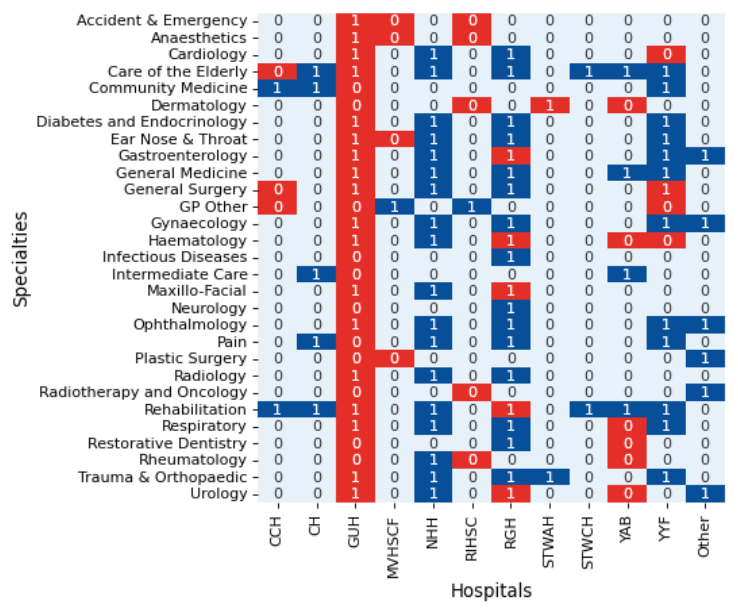
\includegraphics[scale=0.7]{Chapters/Chapter6/Figures/UpdatedSpec.png}
    \caption{Hospitals and Specialties in ABUHB, with 1 Indicating a Specialty is Present in a Given Hospital. For Cells with a \textcolor{red}{Red} Background Displays Where Specialties Have Opened or Closed.}
    \label{fig:relocation}
\end{figure}

In order to incorporate GUH into the model with the existing data, the assumption has been made that patients will be admitted to any hospital within the healthboard and the regional restrictions are lifted. This results in the following constraints, where the $D_{s,r}$ parameter is changed to $D_{s}$:\\
\underline{Deterministic Model}
\begin{equation}
    \sum_{h\in\mathcal{H}} x^\textnormal{bed}_{s,h}\geq D_{s}  \hspace{0.5cm} \forall  s \in \mathcal{S}
\end{equation}
\underline{Two-Stage Stochastic Model}
\begin{equation}
    \sum_{h\in\mathcal{H}} x^\textnormal{bed}_{s,h} +  \sum_{h\in\mathcal{H}} u^\textnormal{bed}_{s,h,k} \geq D_{s,k} \hspace{0.5cm} \forall s \in \mathcal{S}, k \in \mathcal{K}\\
\end{equation}

%If demand is not met, then in the second stage of the model, a preference matrix ($P_{r,h}$) is introduced to encourage new additional beds to be opened in the same region where the demand is coming from. This preference matrix can then provide a financial penalty if the patients are forced to attend a hospital not in the local region. This additional cost could be from ambulances transferring patients \cite{Axon2015} or ...
%This results in the objective function changing to accommodate this change (Equation \eqref{eq:sto_objectiveupdate}). By adding this parameter as a two-dimensional matrix, it provides the user with the option of increasing the costs for regions further away. Conversely, it also provides the option to have a matrix of ones, where there is no effect on the overall objective function value and there is no penalty. \\
% \underline{Two-Stage Stochastic Model}
% \begin{multline}\label{eq:sto_objectiveupdate}
%     \min \sum_{h\in\mathcal{H}}\sum_{s\in\mathcal{S}}(x^\textnormal{bed}_{s,h}c^\textnormal{bed, 1st}_{s,h} + \sum_{b\in\mathcal{B}}x^\textnormal{staff}_{s,b,h}c^\textnormal{staff, 1st}_{b}) +\\ 
%     \sum_{k\in\mathcal{K}}\sum_{h\in\mathcal{H}}\sum_{s\in\mathcal{S}}p_{k}(\sum_{r\in\mathcal{R}} P_{r,h} u^\textnormal{bed}_{s,h,k}c^\textnormal{bed, 2nd}_{s,h} +
%    \sum_{b\in\mathcal{B}} u^\textnormal{staff}_{s,b,k,h}c^\textnormal{staff, 2nd}_{b})
% \end{multline}

The cost for each Welsh specialty bed was calculated using open source data from Public Health Scotland. The speciality average for the Welsh-generated data was the same as the speciality average for the Scottish-generated data, and the Welsh data also fell inside the Scottish-generated data's specified range. In order to match the average of the Scottish data, new values had to be constructed because the numbers were originally created using the prior hospital/specialty location possibilities without taking GUH into account. If a speciality remains in the same hospital, the previous cost will remain the same. Nonetheless, in some circumstances, hospitals no longer offer as many specialties as they once did, falling short of the Scottish average. As a result, these values are altered to conform to the average. The final values for $c^\textnormal{bed,1st}_{s,h}$ and $c^\textnormal{bed,2nd}_{s,h}$ can be seen within Table \ref{tab:appscenariodata}. Similarly, since the opening of GUH, the number of available beds within existing hospitals have decreased. GUH has an available 560 beds within the hospital available to all patients, however the number has been scaled down to 300 to take the age group into consideration. Because fewer beds are available, this has an impact on the K$_{s,h}$, UB$^\textnormal{max, bed, 1st}_{h}$ and UB$^\textnormal{max, bed, 2nd}_{h}$ variables. Once more, this is depicted in Table \ref{tab:appscenariodata}.

%To encourage patients to be admitted to the hospital within a region they reside, a preference matrix can be introduced. The hospital is penalised if patients attend a hospital not in the local region.

%As the regression tree nodes \hl{resulted} in similar results to the OpenSolver averages, this method will be used to generate the demands moving forward. By linking the predictive and prescriptive paradigms, the scenario analysis can utilise more specific scenarios by varying the demand through nodes individually. This is more realistic than the current practice of increasing and decreasing the demands by a fixed percentage. The data will be used over a the entire three years worth of data. Even though more savings can be made if planned on a smaller scale, i.e., yearly, it is impractical to for the healthboard to make such changes on a regular scale.

Initially, running the model with the four scenarios as previously indicated yields a deterministic value of $\pounds$753,963.68 with the deployment of 981 beds and 489 staff (Table \ref{tab:Scenario1Results}). In the case of the two-stage stochastic model, this amount rises to $\pounds$774,285.16. These findings demonstrate that establishing GUH and redesigning the specialties within hospitals resulted in financial savings of approximately $\pounds$200,000. This shows the benefit to decision makers of opening this hospital, and the savings they can potentially make by using the two-stage stochastic model (2.70\%).


\begin{table}[h!]
    \centering
    \begin{tabular}{cccccl}\toprule
 & \multicolumn{2}{l}{\textbf{Total Beds}} & \multicolumn{2}{c}{\textbf{Total Staff}} & \multirow{2}{*}{\textbf{Objective Value ($\pounds$)}}\\ \cmidrule(lr){2-3} \cmidrule(lr){4-5}
         
 & xbed           & ubed          & xstaff         & ustaff         \\ \midrule
 Deterministic & 982 & - & 489 & - & $\pounds$753,963.68 = EV \\
 Stochastic & 940 & 136 & 462 & 75 & $\pounds$774,285.16 = RP \\
 Test A & 981 & 94 & 489 & 69 & $\pounds$791,998.70
 = EEV \\\bottomrule
    \end{tabular}
    \caption{Deterministic and Two-Stage Stochastic Results - Scenario 1}
    \label{tab:Scenario1Results}
\end{table}

%The models presented will also be more generalised to the healthboard

%Using Table \ref{} \hl{Reference} from within the Appendix
% The specific nodes can have values increased or decreased as to what potential future scenarios are likely to involve, rather than simply increasing or decreasing the overall demand. 




%\subsection{Adding in Grange}
% The final scenario investigates the effect on current services if a new hospital is added into the region. Within ABUHB a specialist critical care centre known as The Grange University Hospital, was opened in 2022, (\hl{check}), with the aim to centralise existing services within the healthboard. Therefore

%\hl{think I can merge these two together?}
%\subsection{Flexibility in moving patients to different regions}
% \begin{itemize}
%     \item How would services work if there was an overlap, with a Preference matrix to allow movement between services - maybe? 
% \end{itemize}
\subsection{M-Penalty}\label{sec:scenario2}
The models so far have only considered hard constraints. Hard constraints are where constraints must be satisfied by any feasible solution to produce an optimal solution. However, in reality, if there is not sufficient capacity, patients cannot be admitted into hospitals and either treated at home, or transferred to a neighbouring healthboard for treatment. This situation would then result in an additional cost. The penalty can be incorporated into the existing constraints by the addition of the decision variable $z$, where $z \in \mathbb{N}$. In order to account for this within the objective function, a cost term of $M$ is added, where $M$ is a fixed cost regardless of hospital or specialty. If this was to made more specific to the specialty or hospital, the subscripts $_{s,h}$ could be added and a two-dimensional variable generated. The objective value function and first constraint are thus formulated as follows.

\underline{Deterministic Model}
\begin{equation}\label{eq:det_objective}
    \min \sum_{h\in\mathcal{H}}\sum_{s\in\mathcal{S}}(x^\textnormal{bed}_{s,h}c^\textnormal{bed}_{s,h} + \sum_{b\in\mathcal{B}}x^\textnormal{staff}_{s,b,h}c^\textnormal{staff}_{b}) + Mz
\end{equation}
\begin{equation}
    \sum_{h\in\mathcal{H}} x^\textnormal{bed}_{s,h}\geq D_{s} + z \hspace{0.5cm} \forall  s \in \mathcal{S}
\end{equation}
\underline{Two-Stage Stochastic Model}

\begin{multline}\label{eq:sto_objectiveupdate}
    \min \sum_{h\in\mathcal{H}}\sum_{s\in\mathcal{S}}(x^\textnormal{bed}_{s,h}c^\textnormal{bed, 1st}_{s,h} + \sum_{b\in\mathcal{B}}x^\textnormal{staff}_{s,b,h}c^\textnormal{staff, 1st}_{b}) +\\ 
    \sum_{k\in\mathcal{K}}\sum_{h\in\mathcal{H}}\sum_{s\in\mathcal{S}}p_{k}(u^\textnormal{bed}_{s,h,k}c^\textnormal{bed, 2nd}_{s,h} +
   \sum_{b\in\mathcal{B}} u^\textnormal{staff}_{s,b,k,h}c^\textnormal{staff, 2nd}_{b}) + Mz
\end{multline}

\begin{equation}
    \sum_{h\in\mathcal{H}} x^\textnormal{bed}_{s,h} +  \sum_{h\in\mathcal{H}} u^\textnormal{bed}_{s,h,k} \geq D_{s,k} \hspace{0.5cm} \forall s \in \mathcal{S}, k \in \mathcal{K}\\
\end{equation}

These new objective functions and constraints can be inputted into the OpenSolver model and solved with the regression tree nodes as demands. Since hard constraints have been used previously, the model will produce the same results as those in Section \ref{{sec:scenario1}} and the objective function values shown in Table \ref{tab:Scenario1Results}. However, if hospital beds are reallocated to other patient age groups within the hospital, or decision makers decide to close hospitals, or specialties within certain hospitals, testing will be necessary to ascertain the effects on overall costs and resource requirements.


If decision makers decided to reduce the number of available beds within STWAH to elderly and frail patients, then this would cause the services of dermatology and T\&O to close within this hospital. Although T\&O services can be transferred to RGH, GUH, NHH or YYF, no other hospital offers dermatology treatments. Therefore if we make the assumption that dermatology patients would have to be treated at home or at a different healthboard, this would be with an additional cost of $M$.

If we define $M$ as having a value of $\pounds$2,500, this value exceeds all second stage hospital costs throughout the healthboard. It was assumed that $M$ is not scenario dependant meaning that if in one scenario, a penalty occurred, it occurred for all scenarios. Table \ref{tab:Scenario2Results} presents the results of the deterministic and two-stage stochastic models. The healthboard received a deterministic outcome that allocated 979 beds and 486 nurses, yielding an EV of $\pounds$757,345.32. This value contains an average daily cost of $\pounds$7,500, where three dermatology beds are required but the demand cannot be met, i.e. $z=3$. By closing this hospital to the elderly and frail, this causes a 0.45\% increase in daily costs, equivalent to $\pounds$3,381.64 when compared to Table \ref{tab:Scenario1Results}. The two-stage stochastic model involves the deployment of 936 beds in the first stage and a maximum of 150 beds in the second stage. This increases the objective value to $\pounds$770,181.90, an decrease of 0.53\% without using the M-penalty method. The VSS can be calculated to be 3.28\% with an additional saving of $\pounds$25,258.74 per day by using the stochastic solution over the deterministic.

\begin{table}[h!]
    \centering
    \begin{tabular}{cccccl}\toprule
 & \multicolumn{2}{l}{\textbf{Total Beds}} & \multicolumn{2}{c}{\textbf{Total Staff}} & \multirow{2}{*}{\textbf{Objective Value ($\pounds$)}}\\ \cmidrule(lr){2-3} \cmidrule(lr){4-5}
         
 & xbed           & ubed          & xstaff         & ustaff         \\ \midrule
 Deterministic & 979  & - & 486 & - &$\pounds$757,345.32 = EV \\
 Stochastic & 936 & 150 & 459 & 75 & $\pounds$770,181.90 = RP \\
 Test A & 979 & 93 & 486 & 69 & $\pounds$795,440.64 = EEV \\\bottomrule
    \end{tabular}
    \caption{Deterministic and Two-Stage Stochastic Results - Scenario 2}
    \label{tab:Scenario2Results}
\end{table}


The greatest effects of the M-penalty can be seen within Section \ref{sec:scenario4}, where the demands have be increased significantly to simulate the effects of a pandemic similar to those of Covid-19 to determine the robustness of the healthcare system.

\subsection{Re-evaluating the Current Setup}\label{sec:scenario3}
This section aims to re-evaluate the current arrangement of specialties bed sites in the healthboard and to ascertain the most effective method of specialty reorganisation. This operates under the assumption that a patient can be admitted to any hospital within the healthboard and that every hospital has the capability of having any speciality. Since the opening of GUH in 2020, specialties have been rearranged around the healthboard. This work will determine the most efficient way to organise beds and nursing staff in order to meet the current demand.

The models will operate under the premise that patients can be admitted into any local hospital (Section \ref{sec:scenario1}) and that there is a penalty (Section \ref{sec:scenario2}) if demand is not satisfied throughout the healthboard.

Previously, specialty bed costs from Public Health Scotland have been utilised for the models (Table \ref{tab:PHSCostsPerSpecialty}). %These variables will be extended to provide a cost for every specialty in every hospital.
% Recall Table \ref{tab:PHSCostsPerSpecialty2} which contains the range of costs from Public Health Scotland for specialties within the healthboard.
As this scenario allows all hospitals to have all specialties, the cost matrix for first and second stage beds requires modifying to incorporate this. The prior costings will be recalculated using the new values for each hospital and speciality that fall within the specified ranges, with the average being set at the average of the Scottish data. Table \ref{} \hl{REFERENCE} within the Appendix depicts these newly generated figures. If a hospital already has a speciality, the cost was applied just like in the preceding instance.

Table \ref{tab:Scenario3Results} displays the final figures once the model has been executed. Within this model, 982 beds are deployed with 492 nursing staff required. In the majority of cases specialities are localised to one or two hospitals (Figure \ref{} \hl{APPENDIX FIGURE}). To deploy the specialty of T\&O, three hospitals are required and for rehabilitation specialty four hospitals are required. There is no overlap between these two specialities, therefore if a hospital has a T\&O ward, they would not have a rehabilitation ward. The VSS is calculated to be 3.64\%, showing the benefit of utilising the stochastic model over the deterministic model.

\begin{table}[h!]
    \centering
    \begin{tabular}{cccccl}\toprule
 & \multicolumn{2}{l}{\textbf{Total Beds}} & \multicolumn{2}{c}{\textbf{Total Staff}} & \multirow{2}{*}{\textbf{Objective Value ($\pounds$)}}\\ \cmidrule(lr){2-3} \cmidrule(lr){4-5}
         
 & xbed           & ubed          & xstaff         & ustaff         \\ \midrule
 Deterministic & 982  & - & 492 & - &$\pounds$638,902.04 = EV \\
 Stochastic & 952 & 148 & 468 & 72 & $\pounds$644,663.86 = RP \\
 Test A & 982 & 98 & 492 & 69 & $\pounds$668,112.26 = EEV \\\bottomrule
    \end{tabular}
    \caption{Deterministic and Two-Stage Stochastic Results - Scenario 3}
    \label{tab:Scenario3Results}
\end{table}

\subsection{Long term predictions}\label{sec:scenario4}
Long-term planning decisions in healthcare are critical in determining how demand will fluctuate or change in the future. There are four main reasons as to why long term planning is essential:
\begin{enumerate}
    \item Anticipation of future needs: Long-term planning helps healthcare organisations to anticipate future needs and plan accordingly. Healthcare providers can plan to extend certain services that are suited to the requirements of the elderly, such as COTE, if an area is experiencing an ageing population.
    \item Financial stability: The NHS has a limited spending budget per year assigned by the Government. By planning for future demand and capacity, decision makers can ensure they have the resources needed, without overspending and to continue to provide quality care.
    \item Improved patient outcomes: Long-term planning can allow healthcare organisations to focus on preventative measures and early intervention. By anticipating future healthcare needs, organisations can develop strategies to address them proactively, leading to better health outcomes for patients.
    \item Resource allocation: Long-term planning allows healthcare organisations to allocate resources effectively. With this planning, decision makers can make informed decisions about where to invest resources, such as building new healthcare facilities, hiring additional staff or purchasing new equipment.
\end{enumerate}

These reasons highlight how critical it is for the NHS being able to adapt to change. The demand and pressures on the NHS are expected to increase over the coming years due to rising populations \cite{WelshGovernment2022b}, Covid-19 recovery backlog \cite{AGW2022} and lifestyle factors that lead to an increase in hospital admissions \cite{Luben2019}. 

The impact of a reduction in the number of staff members available is examined in the following scenario. There are several reasons why this might happen, including nurses leaving their jobs after the Covid-19 pandemic \cite{Devereux2022}, nurses taking industrial action for fairer pay and working conditions \cite{RCN2023} or due to sickness \cite{WelshGovernment2022a}.

If we make the assumption the number of nursing staff available reduced to 160 for each band in the first stage, and an additional 40 available within the second stage, the EV produced a value of $\pounds$755,586.60. Due to the limited availability of staff, it caused the $z$ decision variable to be equal to three, as wards could not open as they did not meet the safe staffing levels. %Most interestingly, the stochastic model does not meet the optimal value within the 100 second time limit and causes a non-optimal number of staff to be deployed in a number of cases.
% Within the EEV solution, the $z$ decision variable is also equal to three, meaning in the stochastic environment, the model is able to reduce the penalty face by not meeting this demand. 
The VSS was calculated to be 3.50\% with daily savings of $\pounds$26,824.82. The location of where beds should be deployed in this scenario can be seen in Figures \ref{} \hl{Reference}.

\begin{table}[h!]
    \centering
    \begin{tabular}{cccccl}\toprule
 & \multicolumn{2}{l}{\textbf{Total Beds}} & \multicolumn{2}{c}{\textbf{Total Staff}} & \multirow{2}{*}{\textbf{Objective Value ($\pounds$)}}\\ \cmidrule(lr){2-3} \cmidrule(lr){4-5}
         
 & xbed           & ubed          & xstaff         & ustaff         \\ \midrule
 Deterministic & 979 & - & 480 & - &$\pounds$755,586.60 = EV \\
 Stochastic & 942 & 134 & 462 & 72 & $\pounds$766,801.30 = RP \\
 Test A & 979 & 94 & 480 & 69 & $\pounds$793,626.12 = EEV \\\bottomrule
    \end{tabular}
    \caption{Deterministic and Two-Stage Stochastic Results - Scenario 4}
    \label{tab:Scenario4Results}
\end{table}



% There are three main causes for why the demand will change in the future. Firstly, as Wales has an ageing population, it is expected the number of people falling into the 65 and over category will increase. Therefore the amount of patients 

% This section will look at increasing the demands for demand for the individual nodes, 

% % Firstly, if we keep the demands the same, but reduce the number of staff available either due to sickness \cite{} or strike action \cite{} \hl{REFERENCE}. If we make the assumption there are 160 nursing staff available for each specialty in the first stage, and an additional 40 available within the second stage, produces an EV value of $\pounds$7,.. This causes a total sum for $z$ to be \hl{X}, as wards cannot open as they do not meet the safe staff levels

% \begin{table}[h!]
%     \centering
%     \begin{tabular}{cccccl}\toprule
%  & \multicolumn{2}{l}{\textbf{Total Beds}} & \multicolumn{2}{c}{\textbf{Total Staff}} & \multirow{2}{*}{\textbf{Objective Value ($\pounds$)}}\\ \cmidrule(lr){2-3} \cmidrule(lr){4-5}
         
%  & xbed           & ubed          & xstaff         & ustaff         \\ \midrule
%  Deterministic &   & - &  & - &$\pounds$ = EV \\
%  Stochastic &  &  &  &  & $\pounds$ = RP \\
%  Test A &  &  &  &  & $\pounds$ = EEV \\\bottomrule
%     \end{tabular}
%     \caption{Deterministic and Two-Stage Stochastic Results - Scenario 4}
%     \label{tab:Scenario4Results}
% \end{table}


% This model will look at three experiments where 

% As this data

As the regression tree nodes resulted in similar results to the OpenSolver averages, this method will be used to generate the demands moving forward. The scenario analysis can use more particular scenarios by modifying the demand through individual nodes by linking the predictive and prescriptive paradigms. This is more realistic than the current practice of increasing and decreasing the demands by a fixed percentage. The complete three years' worth of data will be utilised. Although more savings could be achieved by planning on a smaller time frame, such as annually, it would be impracticable for the healthboard to implement such adjustments frequently. There will be two long-term prediction scenarios examined. The first will investigate how the introduction of virtual wards could reduce demand, while the second will analyse a sudden increase in demand.

It is well-known within the medical community that patients who receive care at home recover quicker \cite{CHNFT2022}. This can be due to more support from family members and care-givers or less risk of infection. A new development in healthcare are virtual hospital wards, which came forth in response to the Covid-19 pandemic. With the support of these wards, patients can obtain treatment and monitoring in the convenience of their own homes, lessening the strain on hospitals and lowering the risk of contracting Covid-19. With the use of various digital technologies, virtual hospital wards can offer patients remote monitoring, doctor consultations, and access to medical supplies and medications. This approach to healthcare delivery has the potential to revolutionise the way practitioners provide care to patients, particularly those with chronic conditions, and enhancing patient outcomes while reducing healthcare costs. Virtual wards can be used to discharge patients more quickly or prevent them from being admitted at all \cite{Trueland2023}.

If ABUHB were to implement similar virtual wards as adopted in other regions of the UK, this could provide numerous benefits. Cardiology and respiratory care are two of the disciplines where the Croydon Health Services NHS Trust has implemented virtual wards \cite{HINSL2021}. The trust found cost savings of approximately $\pounds$1,080 per patient, and only 20\% of patients were required to be admitted to hospital. This can be applied to ABUHB by decreasing the demand for cardiology and respiratory services in one scenario by 10\% and in another scenario by 30\%.%by a number of percentages as shown in Table \ref{tab:scenarios2}.

The deterministic demand remains unchanged as if there was no implementation by decision makers to add in virtual wards to the hospitals. This results in the deterministic model produced an objective value of $\pounds$757,345.32 (Table \ref{tab:Scenario6Results}). The two scenarios within the stochastic model reduce the number of beds and staff required to be deployed to a maximum of 970 beds and 480 staff, generated an objective value of $\pounds$751,282.60. This shows that a potential daily saving of $\pounds$6,062.72 if the demand on cardiology and respiratory services were to decline. This highlights the advantages of virtual wards and enables decision-makers to assess its viability from a financial and logistical standpoint.

\begin{table}[h!]
    \centering
    \begin{tabular}{cccccl}\toprule
 & \multicolumn{2}{l}{\textbf{Total Beds}} & \multicolumn{2}{c}{\textbf{Total Staff}} & \multirow{2}{*}{\textbf{Objective Value ($\pounds$)}}\\ \cmidrule(lr){2-3} \cmidrule(lr){4-5}
         
 & xbed           & ubed          & xstaff         & ustaff         \\ \midrule
 Deterministic & 979  & - & 480 & - &$\pounds$757,345.32 = EV \\
 Stochastic & 970 & 0 & 480 & 0 & $\pounds$751,282.60 = RP \\
 Test A & 979 & 0 & 480 & 0 & $\pounds$757,345.32 = EEV \\\bottomrule
    \end{tabular}
    \caption{Deterministic and Two-Stage Stochastic Results - Scenario 3}
    \label{tab:Scenario6Results}
\end{table}

In January 2020, Covid-19 was declared a Public Health Emergency of International Concern, with this being characterised as a pandemic on the 11$^{th}$ March 2020 \cite{WHO2023}. This caused sudden and extreme pressure on the NHS which was already under previous stress from inadequate planning and under-resourcing \cite{BMA2022}. The next scenario will consider how the model will cope in another similar pandemic situation. The deterministic model will utilise the normal regression demand, with the scenarios considering if demand across all specialties and hospitals increased by 20\% and 40\%.

Table \ref{tab:Scenario7Results} presents the results if demand were to suddenly increase and appropriate planning had not taken place. The objective value increase by 35\% in the stochastic model compared to the deterministic model. This is a large increase of unexpected demand with the total number of beds increasing by up to 378. The VSS produces a value of 2.14\%, with the objective function almost twice the value of the deterministic model. 
\begin{table}[h!]
    \centering
    \begin{tabular}{cccccl}\toprule
 & \multicolumn{2}{l}{\textbf{Total Beds}} & \multicolumn{2}{c}{\textbf{Total Staff}} & \multirow{2}{*}{\textbf{Objective Value ($\pounds$)}}\\ \cmidrule(lr){2-3} \cmidrule(lr){4-5}
         
 & xbed           & ubed          & xstaff         & ustaff         \\ \midrule
 Deterministic & 979  & - & 480 & - &$\pounds$757,345.32 = EV \\
 Stochastic & 1176 & 181 & 573 & 90 & $\pounds$1,023,409.16 = RP \\
 Test A & 979 & 444 & 480 & 201 & $\pounds$1,045,268.96= EEV \\\bottomrule
    \end{tabular}
    \caption{Deterministic and Two-Stage Stochastic Results - Scenario 3}
    \label{tab:Scenario7Results}
\end{table}


This section has provided an overview of a variety of scenarios the models are able to plan for. This can aid decision makers when planning services by determining how beds and staff would need to be planned for the future. Whilst tailored to specific questions determined by ABUHB, the flexibility within the model allows the user to apply this to other scenarios they may wish to investigate.



\section{Generalisability of results}\label{sec:generalization}

Generalising results is a critical aspect of research that helps to ensure that the findings of a study are relevant and applicable beyond the specific context in which they were obtained. This makes it possible to guarantee that the study will be beneficial and instructive for other academics, professionals, and policymakers who could be working in other locations or with various populations. Also, generalising findings contributes to a study's external validity, which is crucial for creating a solid body of scientific knowledge.

Both Microsoft Excel and Python implementations have been supplied, in Chapter \ref{chp:tool} and are available on GitHub \cite{}\hl{REFERENCE}, in order to make the models flexible for use by other researchers and healthcare specialists. Excel's OpenSolver was adopted since it can be utilised by staff at all levels within the ABUHB and does not require any prior programming skills. The healthboard's data is conveniently saved in Microsoft Excel files, making it easy for users to enter their data into the model. The Python model is also provided because it is flexible, allowing users to make changes quickly and simply, in response to evolving data or requirements. Because of its versatility, the model can still make precise predictions as more data becomes available. Furthermore, an adaptable Python model allows for more efficient experimentation and testing, as it can be quickly adjusted and re-run with different parameters. To ensure users are able to apply this to their own work, Chapter \ref{chp:tool} provides a tutorial on how to utilise both models.

The deterministic and two-stage stochastic equations are able to be applied to any healthcare scenario. Whilst this research particularly focused on elderly and frail patients, due to the changing population demographics within the healthboard, the equations can be applied to other age groupings. The benefit of using CART models is that researchers and clinicians can apply the theory to their own patient types and identify distinctive homogeneous clusters of patient features. As time passes and the demographic of patients change, these models can be rerun to determine new patient clusters. The user can choose the number of hospitals in each region and the range of specialties they may provide because of the equations' structure, which allows the models to be adjusted to fit any size healthboard. Whilst these models were run with three levels of nursing bands, these can be increased or decreased to suit the user. Additionally, if decision makers wanted to determine the needs for other resources for hospitals such as ventilators, these could be easily added into the model. The models are adaptable and reliable to suit a variety of healthcare situations.

% \begin{itemize}
% \item Excel tool has been provided - for healthboard in Chap
% \item Python Tool has been provided to enable different specailties  hospitals etc.
%     \item Model is adaptable
%     \item used for any healthboard region size
%     \item applied to other age groupings - esp with cart as this can determine different los groupings
%     \item 
% \end{itemize}

\section{Summary}
By linking predictive and prescriptive analytics, decision makers can obtain a comprehensive view of their data and use it to make better decisions. For example, if predictive analytics indicates there is a high likelihood of a certain event occurring in the future, prescriptive analytics can recommend specific actions that can be taken to mitigate the risk or take advantage of the opportunity. Furthermore, this integration can also allow decision makers to continuously improve their decision-making processes over time. By tracking the effectiveness of their decisions and making adjustments based on new data and insights, they can optimise their operations and achieve better outcomes.

This chapter has discussed how predictive and prescriptive analytics could be used in combination for efficiently planning hospital specialty beds and staffing requirements for a network of hospitals in South East Wales. By comparing the regression tree and classification results to the averages, allowed differences to be determined and validation of the linked methods to take place. The results showed regression trees produced closer results to the averages. The validation of these regression trees paves the way for more complex scenario analysis. The addition of GUH, adding a soft constraint penalty and determining future scenarios were three main avenues explored. These results showed the potential and robustness of the models, which enables them to be applied to future scenarios that healthboard may wish to investigate. The models are also generalisable so can be applied to any age demographic or hospital region and therefore can be used in other aspects of ABUHB and applied to worldwide healthcare organisations.

In the following chapter, Chapter \ref{chp:tool}, a tutorial is provided on how to use the Microsoft Excel OpenSolver and the Python PuLP tools.


\end{document}
